\documentclass[tikz,border=3pt]{standalone}
\usepackage[utf8]{inputenc}
\usepackage[T1]{fontenc}
\usepackage{lmodern}
\renewcommand{\familydefault}{\sfdefault}
\usepackage{sansmath}\sansmath
\usepackage{chemfig}
\usepackage{pgfplots}\pgfplotsset{compat=1.18,/pgf/number format/use comma,/pgf/number format/1000 sep={.}}
\usetikzlibrary{arrows.meta,calc,positioning,decorations.pathmorphing,patterns}
% paleta del sitio
\definecolor{nar}{HTML}{E8680C}\definecolor{narc}{HTML}{FFB35C}\definecolor{hielo}{HTML}{FFF3E8}
\definecolor{tinta}{HTML}{1D1D1F}\definecolor{gris}{HTML}{6E6E73}\definecolor{lila}{HTML}{7C5CF0}
\definecolor{azul}{HTML}{2F6FD6}\definecolor{menta}{HTML}{17A673}\definecolor{coral}{HTML}{E8342A}
\begin{document}
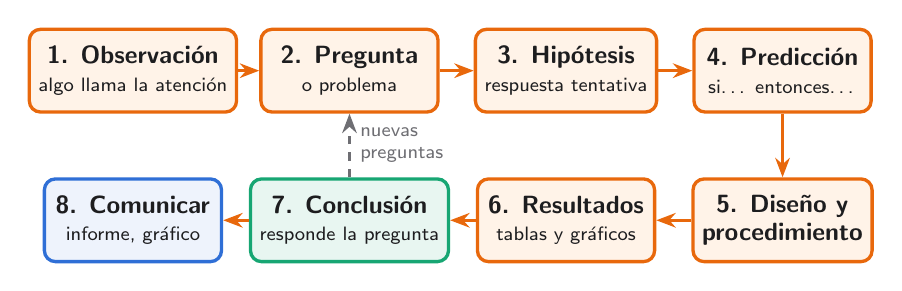
\begin{tikzpicture}[font=\small,
  caja/.style={draw=nar,very thick,fill=hielo,rounded corners=4pt,minimum width=2.25cm,minimum height=1.05cm,align=center,text=tinta},
  flecha/.style={-{Stealth[length=7pt]},very thick,nar}]
\node[caja] (obs) at (0,0) {\textbf{1. Observación}\\[-1pt]{\scriptsize algo llama la atención}};
\node[caja] (pre) at (2.75,0) {\textbf{2. Pregunta}\\[-1pt]{\scriptsize o problema}};
\node[caja] (hip) at (5.5,0) {\textbf{3. Hipótesis}\\[-1pt]{\scriptsize respuesta tentativa}};
\node[caja] (pred) at (8.25,0) {\textbf{4. Predicción}\\[-1pt]{\scriptsize si\ldots\ entonces\ldots}};
\node[caja] (dis) at (8.25,-1.9) {\textbf{5. Diseño y}\\[-1pt]\textbf{procedimiento}};
\node[caja] (res) at (5.5,-1.9) {\textbf{6. Resultados}\\[-1pt]{\scriptsize tablas y gráficos}};
\node[caja,draw=menta,fill=menta!10] (con) at (2.75,-1.9) {\textbf{7. Conclusión}\\[-1pt]{\scriptsize responde la pregunta}};
\node[caja,draw=azul,fill=azul!8] (com) at (0,-1.9) {\textbf{8. Comunicar}\\[-1pt]{\scriptsize informe, gráfico}};
\draw[flecha] (obs) -- (pre);
\draw[flecha] (pre) -- (hip);
\draw[flecha] (hip) -- (pred);
\draw[flecha] (pred) -- (dis);
\draw[flecha] (dis) -- (res);
\draw[flecha] (res) -- (con);
\draw[flecha] (con) -- (com);
\draw[flecha,dashed,gris] (con.north) -- node[right,font=\scriptsize,text=gris,align=left] {nuevas\\preguntas} (pre.south);
\end{tikzpicture}
\end{document}
